\documentclass{article}
\usepackage[margin=1in]{geometry}
\usepackage{hyperref} % for links and URLs
\usepackage{longtable} % for displaying command-line parameters
\usepackage{bibentry} % for having bibliographic entries appear in--text
\usepackage{graphicx} % trivial image display
\usepackage{listings} % for writing XML to represent the DNA motif schema
\usepackage{color}
\hypersetup{colorlinks=true, linkcolor=red}

\begin{document}

% Create main front page
\title{Marina -- Using several statistical metrics to identify over--represented 
transcription factor binding sites. \\ \small{Marina version 1.01 -- Documentation \& Tutorial}}
\author{Parsa Hosseini}
\maketitle
\tableofcontents % Have TOC on the main front page
\pagebreak

% --- Introduction ---
\section{Introduction}
\subsection{What Marina is and is not}
\texttt{Marina} is a GUI software tool for identifying over--represented transcription factor
binding sites (TFBS) through the use of several knowledge--discovery / data--mining metrics. 
These metrics quantify and normalize TFBS abundance, ultimately producing a 
standardized rank of each TFBS and its magnitude of over--representation. Since
multiple metrics are involved, a normalization algorithm known as 
Iterative Proportional Fitting (IPF) is used to yield ``agreement'' across all
metrics as--to which TFBSs are truly the most over--represented.

\texttt{Marina} is not a centralized database of TFBSs much like that of TRANSFAC, 
AthaMap, AGRIS, amongst others. Rather, \texttt{Marina} is built for an 
investigator to efficiently mine promoter sequences and find
statistically--sound and over--represented TFBSs across multiple groups of promoter-sequence sets.

\subsection{Marina prerequisites}
Prior to version 1.00, \texttt{Marina} was built using the Python programming
language. Since then, this software has been re--built from the ground up using
the Java programming language. Several major fixes are present in this latest
build and we encourage usage of this over prior Python builds.
\begin{itemize}
  \item[-] Java (version 7+ recommended) \url{http://www.java.com}
  \item[-] x86 or x64 system with Linux, Mac or Windows OS.
\end{itemize}


\subsubsection{Abbreviations}
\begin{table}[htbc]
	\centering
	\begin{tabular}{c | c }
	\hline Abbreviation & Full name \\ \hline
	CF & Confidence (metric) \\
	CM & Contingency Matrix \\
	CO & Cosine (metric)\\
	IPF & Iterative Proportional Fitting \\
	JAC & Jaccard Index (metric) \\
	JM & J-Measure (metric) \\
	K & Kappa Coefficient (metric) \\
	LI & Lift (metric) \\
	PHI & Phi Coefficient (metric) \\
	PWM & Position Weight Matrix \\
	TFBS & Transcription Factor Binding Site \\
	\end{tabular}
	\caption{List of abbreviations for commonly used terms}
	\label{table:abbreviations}
\end{table}

% --- The underlying data-structures for deducing TFBS over-representation ---
\section{TFBS Quantification and Derivation of Over-Representation}

\subsection{Contingency Matrix}
Central to deriving magnitude of TFBS over--representation to utilization of 
a contingency matrix (CM).
Such a structure is used to model
multivariate frequencies, in our case, TFBS abundance between a baseline and
control set of promoter sequences. Since this data--structure contains discretized counts, these
matrices are frequently used to model magnitude of relationships between a given
set of categorical variables.

\begin{table}[htbc]
	\centering
	\begin{tabular}{c | c | c | c}
	  & $C$    & $\neg{C}$ & \\ \hline
	$x$ & $n(x,C)$ & $n(x,\neg{C})$ & $n(x)$\\
	$\neg{x}$ & $n(\neg{x},C)$ & $n(\neg{x},\neg{C})$ & $n(\neg{x})$\\ \hline
	& $n(C)$ & $n(\neg{C})$ & $N$\\
	\end{tabular}
	\caption{A contingency matrix given a variable of interest, $x$, and a
	categorical variable, $C$}
	\label{table:contigencymatrix}
\end{table}
As illustrated in table \ref{table:contigencymatrix}, frequency counts can be
used to derive relationships given both a variable of interest ($x$)
and a specific categorical variable ($C$). The cumulative sum per row
as well as each column therefore equals that of the entire matrix. 
Indeed a contingency matrix could be extended
to have $i * j$ rows and columns respectively, however \texttt{Marina} utilizes 
a $2*2$ contingency matrix.

\subsubsection{Iterative Proportional Fitting (IPF) algorithm}
\label{section:ipf_algorithm}
An option in \texttt{Marina} is to normalize counts in a contingency matrix so as to
better extract underlying patterns and trends. One algorithm for such a purpose 
is Iterative Proportional Fitting (IPF).
\footnote{Developed by W. E. Demming. On a Least Squares Adjustment of a
Sampled Frequency Table When the Expected Marginal Totals are Known. Annals of
Mathematical Statistics, 1940}
The purpose behind IPF standardization is to adjust cell frequencies 
in such a way that both row and column counts are equal to one
another (see table \ref{table:ipf_matrix}).

\begin{table}[htbc]
	\centering
	\begin{tabular}{c | c | c | c}
	  & $C$    & $\neg{C}$ & \\ \hline
	$x$ & $c(0,0)$ & $c(1,0)$ & $N/2$\\
	$\neg{x}$ & $c(0,1)$ & $c(1,1)$ & $N/2$\\ \hline
	& $N/2$ & $N/2$ & $N$\\
	\end{tabular}
	\caption{IPF adjusts counts in a matrix, c, to aide in identifying inherent
	patterns and associations.}
	\label{table:ipf_matrix}
\end{table}

Upon successful frequency adjustments, a contingency matrix, c, would
exhibit counts satisfying the following patterns: $c_{1,1} = c_{0,0}$, and
$c_{0,1} = c_{1,0}$. This equality pattern is represented in table
\ref{table:ipf_matrix_rev_counts}. Note the monotonic nature of this matrix
given $x$ and $\neg{x}$. 

\begin{table}[htbc]
	\centering
	\begin{tabular}{c | c | c | c}
	  & $C$    & $\neg{C}$ & \\ \hline
	$x$ & $a$ & $N/2 - a$ & $N/2$\\
	$\neg{x}$ & $N/2 - a$ & $a$ & $N/2$\\ \hline
	& $N/2$ & $N/2$ & $N$\\
	\end{tabular}
	\caption{Adjusting a contingency matrix using IPF yields frequency
	counts to aide inherent pattern identification}
	\label{table:ipf_matrix_rev_counts}
\end{table}

As shown in table \ref{table:ipf_matrix_rev_counts} and supported by the two earlier
equality patterns, two equations are needed to populate this matrix
\footnote{As presented by T., P-N. et. al., 'Selecting the right
interestingness measure for association patterns', SIGKDD 2002.}:
\begin{equation}
	c_{1,0} = c_{0,0} = a = \frac{N \sqrt{c_{1,1} c_{0,0}}}
	{2 (\sqrt{c_{1,1} c_{0,0}} + \sqrt{c_{1,0} c_{0,1}} )}
	\label{equation:ipf_first}
\end{equation}

\begin{equation}
	c_{0,1} = c_{1,0} = N/2 - a
	\label{equation:ipf_second}
\end{equation}

Equations \ref{equation:ipf_first} and \ref{equation:ipf_second} present
solutions for populating a matrix all--while satisfying not only previous
equality patterns but also the monotonic nature of the matrix.

\subsection{Metrics for evaluating TFBS over-representation}
\label{section:metrics}
An association rule models dependency between a set of variables, $X$ and $Y$,
defined as $X \rightarrow Y$. We assert that both $X$ and $Y$ occur beyond a
user-defined or default threshold.
Association rules can oftentimes model weak dependencies and as a result,
provide very little novel insight.
Strong dependencies on the other hand deem themselves worthy of detailed attention and
may warrant domain expertise. In other words, a strong association rule implies
occurrence of a variable, $Y$, if $X$ is present. Contingency matrices can model
these very relationships assuming $X$ and $Y$ are discretized variables.

A total of 7 statistical metrics are implemented in \texttt{Marina} to help infer what
TFBSs are over--represented and what are not.
Each of the seven metrics are discussed below, however for an in--depth review of
such metrics, please see \cite{geng-acmcomputing-2006}.

% --- SUPPORT AND CONFIDENCE --- Only used in graph analysis
\subsubsection{Support (SP) \& Confidence (CF)}
\begin{itemize}
  \item \textbf{Metric range:} 0 \ldots 1
\end{itemize}

Support and confidence are two incredibly useful knowledge--discovery metrics. Both
support and confidence were developed by \cite{agrawal-sigmod-1993} and have
come to be one of the most widely--used metrics in data--mining. 
\begin{equation}
	SUPP = \frac{n(x,C)}{N} = P(x,C)
\end{equation}

\begin{equation}
	CONF = \frac{P(x,C)}{P(x)} = P(C| x)
\end{equation}

Many published measures such as Jaccard and Klosgen incorporate both support 
and confidence. Utilization of both these measures was initially proposed by
\cite{kumar-unpublished-2000}. Support and confidence can however generate
a large set of association rule candidates, and unfortunately, many
may not have any significant level of value.

% --- LAPLACE CORRECTION ---
\subsubsection{Laplace Correction (LP)}
\begin{itemize}
  \item \textbf{Metric range:} 0 \ldots 1
\end{itemize}
Laplace correction aims to
quantify magnitude of accuracy for a particular association rule. The $k$
variable in the denominator represents the matrix dimension. As is the case
for a 2x2 contingency matrix, $k=2$. Marina sets a default Laplace correction
cutoff of 0.3; adjusted via the \texttt{-l} or \texttt{--lapl} flag. Items 
bearing higher correction scores would certainly attract more domain--expertise than
lower correction scores.

\begin{equation}
	LP(x, C) = \frac{n(x,C)+1} {n(x) + k}
\end{equation}

% --- LIFT ---
\subsubsection{Lift (LI)}
Otherwise known as interest, lift is a metric developed by
\cite{brin-sigmod-1997}. Lift computes the probability behind $x$ and $C$
occurring together in comparison to if they were independent of one another.
Therefore lift quantifies the reliability behind $x \rightarrow C$. For example: a lift of 3
implies that $x$ is three times as likely to yield $C$ in comparison to what
would be sought under a null hypothesis.
\begin{itemize}
  \item \textbf{Metric range:} 0 \ldots $\infty$
\end{itemize}
\begin{equation}
	LI(x, C) = \frac{P(x, C)}{P(x)P(C)}
\end{equation}

% --- JACCARD INDEX ---
\subsubsection{Jaccard (JAC)}
\begin{itemize}
  \item \textbf{Metric range:} 0 \ldots 1
\end{itemize}
The Jaccard measure \cite{tan-sigkdd-2002} is quite appealing as it incorporates
both support and confidence. When two variables are compared against one
another, if they exhibit similar patterns, the Jaccard metric returns a value
close--to or equal to 1. On the contrary, if the variables are different from one
another, the Jaccard metric yields a much lesser value in the vicinity of 0. The
definition for this metric is shown below:
\begin{equation}
	JAC = \frac{P(x,C)}{P(x)+P(C)-P(x,C)}
\end{equation}

% --- PHI COEFFICIENT ---
\subsubsection{Phi coefficient (PHI)}
\begin{itemize}
  \item \textbf{Metric range:} -1 \ldots 1
\end{itemize}
The phi ($\phi$)--coefficient is a metric to quantitate magnitude of association
given two variables. It is important to note the
difference between ``association'' and ``correlation''. The former implies dependency while the
latter implies a linearly--bound relationship binding two variables. The equation
for computing $\phi$-coefficient given a contingency matrix like that in table
\ref{table:contigencymatrix} is defined below. 

Since the range of this metric is $\pm1$, 
results at these polar--boundaries represent high association between two variables. 
If however a coefficient of zero was obtained, this would represents no inherent relationship.
\begin{equation}
	\phi(x) = \frac{n(x,C)n(\neg{x},\neg{C}) - n(x,\neg{C})n(\neg{x},C)} %numer
		{\sqrt{n(x)n(C)n(\neg{x})n(\neg{C})}} % denom
\end{equation}

% --- COHEN'S KAPPA COEFFICIENT ---
\subsubsection{Kappa Coefficient (K)}
\begin{itemize}
  \item \textbf{Metric range:} -1 \ldots 1
\end{itemize}

\begin{equation}
	\frac{P(x,C)+P(\overline{x,C}) - P(x)P(C) -
        P(\overline{x})P(\overline{C}))}
        {1-P(x)P(C) - P(\overline{x})P(\overline{C})}
\end{equation}

% --- COSINE ---
\subsubsection{Cosine (CO)}
\begin{itemize}
  \item \textbf{Metric range:} 0 \ldots 1
\end{itemize}
Cosine \cite{kumar-unpublished-2000}, also known as Interest--Support (IS), is an
interesting metric for discerning variability given two variables against a null hypothesis. 

\begin{equation}
	CO = \frac{P(x,C)} {\sqrt{P(x)P(C)}}
\end{equation}

% --- How over-represented TFBSs are modeled and evaluated ---
\section{Data Representation}
\label{section:data_repr}
\subsection{Accepted TFBS Models}
As mentioned earlier, a TFBS can modeled in one of two ways (or both, if 
TFBS models are available for each). 
The first representation is in the form of fixed--length DNA sequences, hence 
the name ``DNA motif''. The second model, and most preferred, is known as Position Weight Matrices (PWMs).
Skeleton templates (schemas) for supplying your own TFBS models are described in section \ref{section:custom}.

\subsection{TFBS counts and the hypergeometric distribution (optional)}
\label{section:hypergeometric}
Given the hypergeometric distribution and a TFBS--specific contingency matrix, 
a p-value can be evaluated given TFBS counts across group$_{a}$ and group$_{a+1}$. 
The hypergeometric probability distribution function is as follows:

\begin{equation}
	P(X=k) = \frac{ {M\choose{k}} {{N-M}\choose{n-k}} }{{N\choose{n}}}
	\label{equation:hypergeom}
\end{equation}

As defined in equation \ref{equation:hypergeom}, $x$ represents the random
variable, $N$ is the total population size, $M$ represents the number of
successes given the total population, and $n$ represents the sample size drawn.
As a result, this distribution aims to quantify the probability of $x$
successes from amongst $n$ samples, from population, $N$.
Since we have a populated contingency matrix like that in table
\ref{table:contigencymatrix}, we can work with this matrix to 
yield a hypergeometric distribution probability (table \ref{table:hypergeom}).

Our random variable, $k$, represents the frequency at which $x$ is in group $G$.
On the contrary, $n(\neg{x}, G)$ represents the difference between the number of
trials and the number of successes obtained. Modelling $n(x, \neg{G})$ is however
more complicated since this represents the differences between the number of
successes in the population and number of successes obtained. Marginals can now
be deduced which can aide in filling in the rest of this matrix.

\begin{table}[htbc]
	\centering
	\begin{tabular}{c | c | c | c}
	  & $G$    & $\neg{G}$ & \\ \hline
	$x$ & $k$ & $M - k$ & $M$\\
	$\neg{x}$ & $n - k$ & $N + k - n - M$ & $N - M$\\ \hline
	& $k$ & $N - n$ & $N$\\
	\end{tabular}
	\caption{Transforming a contingency matrix to be modeled by the hypergeometric
	distribution [\href{http://en.wikipedia.org/wiki/Hypergeometric_distribution}{URL}]}
	\label{table:hypergeom}
\end{table}

% --- Schemas for both PWMs and DNA motifs ---
\section{Providing custom PWMs or DNA motifs}
\label{section:custom}
\texttt{Marina} does not come pre-packaged with TFBS models, be--it in the form of
PWMs or DNA motifs.Thankfully, many resources exist containing both these models.
In plants, for instance, several online resources contain useful models which can be imported into 
\texttt{Marina}: AthaMap [\href{http://www.athamap.de/}{URL}], 
JASPAR [\href{http://jaspar.genereg.net/}{URL}], 
TRANSFAC [\href{http://www.gene-regulation.com/pub/databases.html}{URL}],
AGRIS [\href{http://arabidopsis.med.ohio-state.edu/}{URL}], and
PLACE [\href{http://www.dna.affrc.go.jp/PLACE/}{URL}].
Investigators can therefore create their own custom TFBS models given these resources,
assuming licensing and registration requirements are met.

\subsection{Schema for DNA Motifs}
As discussed earlier, there are two models for representing a TFBS. The first being in
the form of a linear string of nucleotide characters, and the latter being as a PWM.
In this section, we discuss the schema of the the former model, DNA motifs.

\begin{lstlisting}[label={motifs},caption=Three-column DNA-motif schema.]
bHLH		OsIRO2		CACGTGG
WHIRLY		StWhy1		GTCAAAAA
ARF		ARF1		TGTCTC
TRIHELIX	GT1-BOX		GTGTGGTTAATATG
TRIHELIX	GT2-BOX		GCGGTAATTAA
TRIHELIX	GT3-BOX		GAGGTAAATCCGCGA
\end{lstlisting}

As shown in listing \ref{motifs}, DNA motifs are represented in a three--column
tab--delimited file. The first column must be a TF family and the second
must represent the TF gene--name. Lastly, the third column represents the actual
TF gene DNA motif (binding site). A collection of literature--derived DNA motifs
are available in the \texttt{/demo/} folder.

\subsection{Schema for PWMs}
\label{section:pwm_schema}
The second way to model a TFBS is through PWMs. Below is an arbitrary example
of a PWM whereby frequency counts are masked as ``x'', cushioned by flanking
braces. These flanking braces are purely optional and are present in the
example below to separate counts in the actual matrix from its respective
nucleotide. PWM data--points are separated from one another by either a 
space or a tab. All elements must also have a corresponding value otherwise
an exception will be thrown at runtime. Similar to sample--DNA motifs, several
sample--PWMs are also available in the \texttt{/demo/} folder.

\begin{verbatim}
>PWM_1
A  [ x  x  x  x  x x  x  x  x ]
C  [ x  x  x  x  x x  x  x  x ]
G  [ x  x  x  x  x x  x  x  x ]
T  [ x  x  x  x  x x  x  x  x ]
...
>PWM_N
A  [ x  x  x  x  x x  x  ]
C  [ x  x  x  x  x x  x  ]
G  [ x  x  x  x  x x  x  ]
T  [ x  x  x  x  x x  x  ]
\end{verbatim}

% --- Tutorial ---
\section{Tutorial}
Assuming \texttt{Marina} was successfully downloaded and all prerequisites
have been met, \texttt{Marina} can be executed 
simply by double--clicking on the ``Marina.jar'' icon or manual execution 
by issuing the command ``java -jar Marina.jar''.
The main GUI will then appear, ready for analysis (Figure \ref{fig:mainGUI}).

To begin analysis, two input conditions must be met: 
\begin{itemize}
  \item 2x FASTA files are required. One of the two will serve as the baseline
  	while the other serves as a query, however both files must contain promoter sequences. 
  	In both files, promoter sequences do not have to be the same length. Similarly,
  	input FASTA files do not have to have the same number of FASTA entries. 
  \item Either DNA motifs or PWMs (or both). These TFBS models are to be mapped
  	onto the 2x user--provided FASTA files. 
\end{itemize}
Sample FASTA files are provided. These files represent promoter sequences of the
most-induced and most-suppressed genes during a Soybean--Soybean Rust
RNA--Seq study(Tremblay et. al, 2012). Sample DNA motifs and PWMs are also provided. 
If you wish to supply your owm motifs, please follow section \ref{section:custom} which outlines
the required schema for providing custom TFBS models.
Both input FASTA files and TFBS models can be supplied through the 
\textbf{File $\rightarrow$ Load FASTA} and \textbf{File $\rightarrow$ Load TFBSs} respectively.

\begin{figure}[htbc]
	\centering
	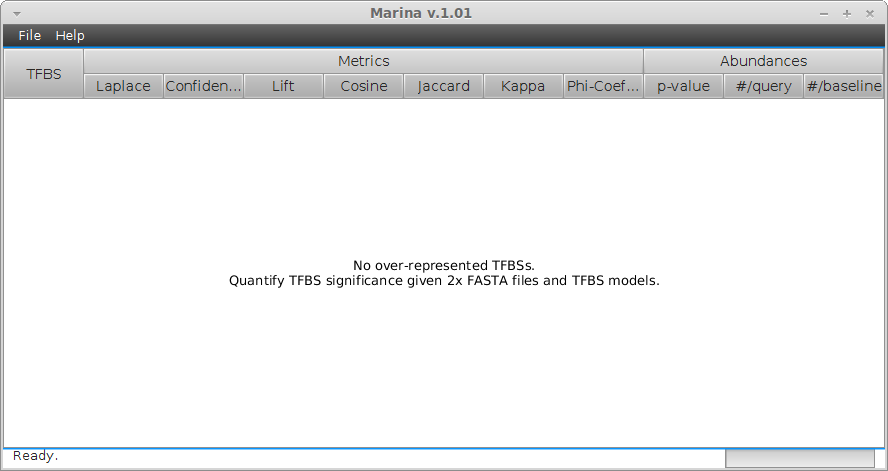
\includegraphics[scale=0.50]{./images/marina_mainGUI.png}
	\caption{GUI upon launching \texttt{Marina}}.
	\label{fig:mainGUI}
\end{figure}

\subsection{Runtime Options}
The investigator can tweak options by going to 
\textbf{File $\rightarrow$ Options} (Figure \ref{fig:marinaOptions}). 
Definition of these parameters are provided in Table \ref{table:params}.
For this tutorial, we will use default arguments.

\begin{figure}[htbc]
	\centering
	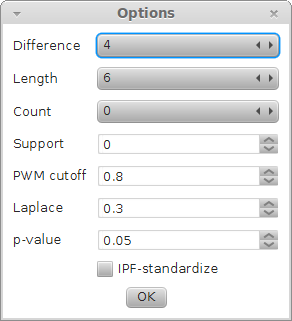
\includegraphics[scale=0.45]{./images/marina_options.png}
	\caption{Options can be modified to provide a more strict or lenient mode of analysis}.
	\label{fig:marinaOptions}
\end{figure}


\begin{longtable}{| p{2.7cm} | c | c | p{8.5cm} |}
	\hline
	Name  & Default & Range & Description \\ \hline \hline
	% Optional parameters -- graph analysis parameters
	\texttt{Difference}  & 4 & 0 \ldots 100 & Represents the
	difference when a graph node's count is compared to its equivalent node in another group.
	Graph nodes with differences less than this are removed.\\
	
	\texttt{Length}  & 6 & 0 \ldots 100 &
	Remove TFBSs that are less than this length.\\

	\texttt{Count}  & 0 & 0 \ldots 100 & Each TFBS is modeled as a graph node
	which is part of a group--specific acyclic graph. Each node has ``count" property
	which is simply the \#/TFBSs mapping to this very node.
	Graph nodes with counts less than this are removed.\\

	\texttt{Support}  & 0 & 0 \ldots 100 & Represents probability a TFBS, $t_i$,
	is in a group, $G_a$. This is otherwise written as $P(t_i, G_a)$.
	All graph nodes having supports less than this are removed. \\

	\texttt{PWM cutoff}  & 0.80 & 0 \ldots 0.99 & Pertains only to when PWMs are supplied.
	When PWMs are mapped onto TFBSs, a probabilistic score is produced; akin to sequence identity.
	Fragments with scores $\geq$ this cutoff are kept.\\

	\texttt{Laplace} & 0.30 & 0 \ldots 0.99 & Several statistical metrics are used for
	evaluating TFBS over--representation. One such metric is Laplace correction (see section
	\ref{section:metrics} for details). This parameter filters
	TFBSs based on their Laplace probability. Lowering this flag may yield many
	TFBSs that may not be over--represented. \\

	\texttt{p-value} & 0.05 & 0 \ldots 0.99 &
	For each over--represented TFBS, an accompanying p-value from the hypergeometric distribution
	is derived. Please refer to section \ref{section:hypergeometric} for detailed workings of this
	distribution. All TFBSs with p-values over this p-value cutoff are 
	filtered--out. \\

	\texttt{IPF--standardize} & False & N/A & Contingency matrices are used to model
	raw--abundance per TFBS given $G_{a}$ and $G_{a+1}$. Standardizing counts within this
	matrix could shed light
	on inherent associations which TFBS abundance between two groups. Such normalization is
	performed via the Iterative Proportional Fitting (IPF) algorithm 
	(see section \ref{section:ipf_algorithm}). \\
	\hline
	\caption{\texttt{Marina} parameters and their respective arguments}
	\label{table:params}
\end{longtable}
\clearpage

\subsection{Running Sample Data}
For this tutorial, we will use files present in the \texttt{/demo/} folder.
We will use both sample motifs and PWMs for this example 
(Table \ref{table:sampleFiles}).
You do not need both PWMs and DNA motifs to begin analysis. This example
uses both models solely to illustrate the ability of \texttt{Marina} to
quantify different TFBS profiles. As long as one of these two models are
provided, that will suffice.

\begin{table}[htbc]
	\centering
	\begin{tabular}{|c|c|c|}
	\hline
		File name & entries & Represents \\ \hline
		most$\_$induced.fasta & 556 & Query \\
		most$\_$suppressed.fasta & 585 & Baseline \\
		sample$\_$motifs.txt & 16 & DNA motifs \\
		sample$\_$pwms.txt & 3 & PWMs \\
	\hline
	\end{tabular}
	\caption{Sample files used for the tutorial}
	\label{table:sampleFiles}
\end{table}

For each of these four files, a success dialog will appear if parsing the
respective file was a success. Exceptions are caught and the investigator is
alerted if the input file was not of an acceptable format. Once these files
have been provided, selecting 
\textbf{File $\rightarrow$ Run $\rightarrow$ Align} will initiate alignment.
If only PWMs were provided, an implementation of the P--MATCH algorithm will be
invoked. Similarly if only DNA motifs were provided, an implementation of the
Rabin--Karp algorithm will be invoked. Since both models are provided, both
alignment algorithms will be executed, back--to--back. Please note that 
prior \texttt{Marina} versions utilized the Boyer--Moore--Horspool algorithm 
for DNA motif alignment.

During analysis, alignment will take place in the background and a progress--bar
will be updated to reflect degree of alignment completion 
(Figure \ref{fig:marina_runtime}). Eventually, alignment will reach completion
and the status--bar will display ``Alignments OK. Ready for quantification.''

\begin{figure}[htbc]
	\centering
	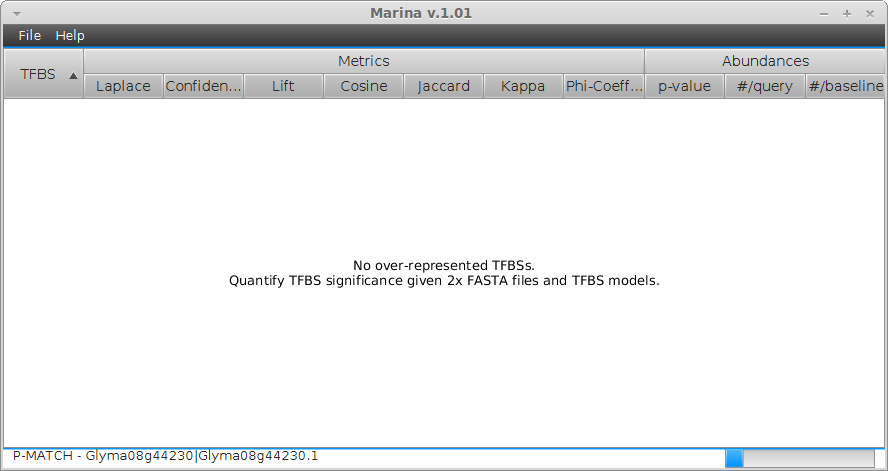
\includegraphics[scale=0.50]{./images/marina_runtime.png}
	\caption{TFBS models being aligned to all provided promoter sequences}.
	\label{fig:marina_runtime}
\end{figure}

Upon alignment completion, we now have reference as to what TFBSs mapped to
what promoter sequences. Given such mappings, we can model TFBS abundances
between the two groups and quantify TFBS magnitude of over--representation.
By selecting \textbf{File $\rightarrow$ Run $\rightarrow$ Quantify}, 
TFBSs are fed through the various options and those which pass all of them
are fed into the 7 statistical metrics (Figure \ref{fig:marina_quantify}). 
Output generated per metric is ranked from 1.0 \ldots $N$, where $N$ represents the total number of over--represented
TFBSs.

\begin{figure}[htbc]
	\centering
	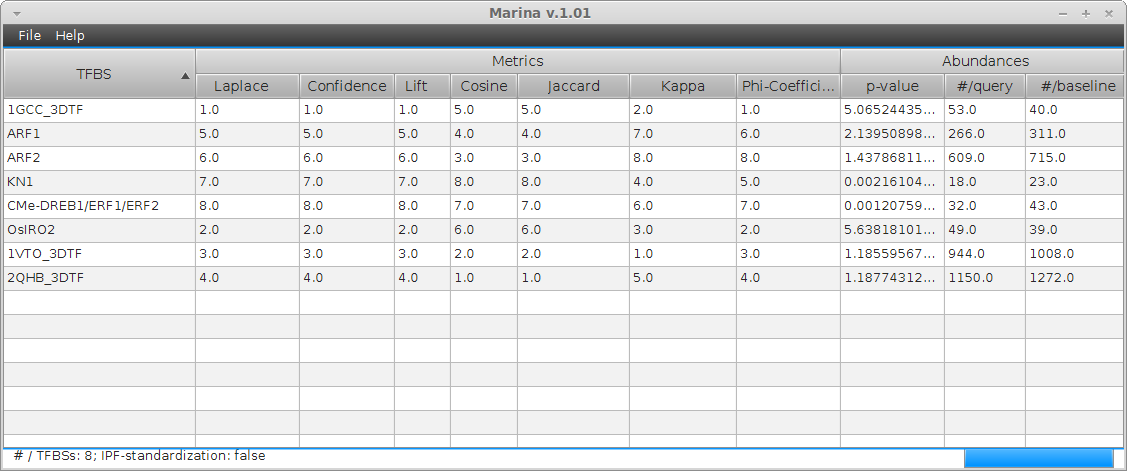
\includegraphics[scale=0.42]{./images/marina_quantified.png}
	\caption{TFBSs with ranks close to 1 are most over--represented and vice--versa}.
	\label{fig:marina_quantify}
\end{figure}

Various metrics may not reach unanimous concensus
as--to the magnitude of over--representation. For instance, ``2QHB$\_$3DTF''
is ranked 1st by 2/7 metrics but ranked 4th by 4/7 and 5th by 1/7. Indeed this
lack of concensus can make identifying the most over--represented TFBSs an
analytical challenge. Had we selected ``IPF--standardize'' in the Options dialog
(Figure \ref{fig:marinaOptions}), the rank per TFBS would be unanimously
agreed--upon by each and every metric (Figure \ref{fig:marina_withipf}).
Results obtained from quantification can saved as a tab--delimited file via. the
\textbf{File $\rightarrow$ Save} option.

\begin{figure}[htbc]
	\centering
	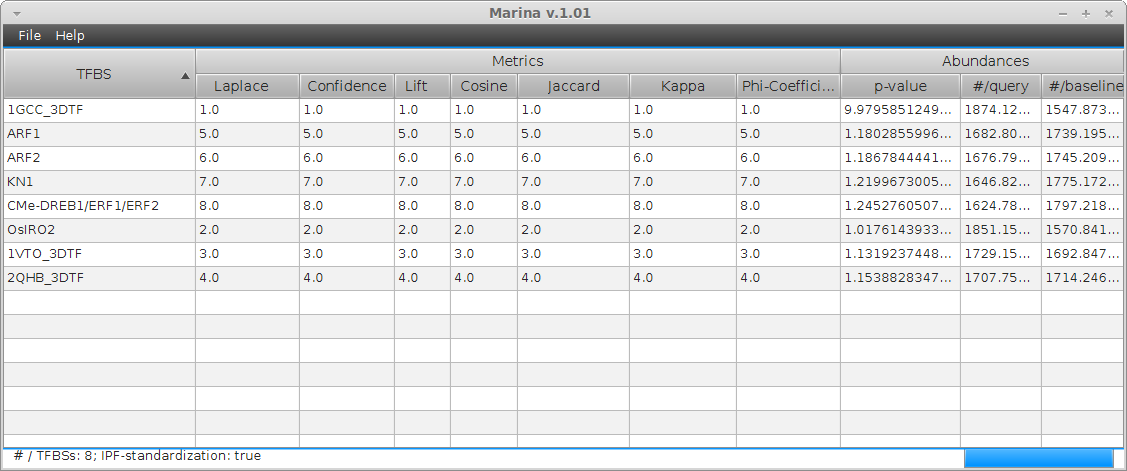
\includegraphics[scale=0.42]{./images/marina_withipf.png}
	\caption{IPF enables all metrics to agree as to which TFBSs are the 
		most over--represented}.
	\label{fig:marina_withipf}
\end{figure}

\section{Questions and Comments}
Please contact Parsa Hosseini (Parsa.Hosseini@ars.usda.gov) if you have
questions or comments about \texttt{Marina} or wish to report a bug.

\clearpage
\renewcommand{\refname}{Useful Resources \& Reading}
\bibliographystyle{alpha}
\bibliography{bib}
\end{document}
